\chapter{Project Logic Diagrams}

\section{Work Flow Diagram}

\section{Work Breakdown Structure}

A Work Breakdown Structure (WBS) is a hierarchical decomposition of a project into smaller, manageable components. It organizes all the work required to deliver a system into clearly defined elements, typically moving from high-level system functions down to detailed tasks or deliverables. The purpose of a WBS is to improve clarity, assign responsibility, support scheduling and budgeting, and ensure that no critical scope is overlooked.

In the case of the unmanned modular test bed, two key aspects were considered when constructing the WBS: the physical system (air vehicle, payload, control), and the mission purpose (experimental testing, replacing conventional wind tunnels). This separation is important because, unlike a conventional aircraft project, the primary output is not the vehicle itself but the data and experimental capability it provides. Testing is elevated from a verification step to a core operational function. This reflects the idea that the platform acts as a “flying laboratory,” addressing limitations of wind tunnels such as mounting interference, scaling constraints, and inability to test to failure.

\begin{figure}[H]
    \centering
    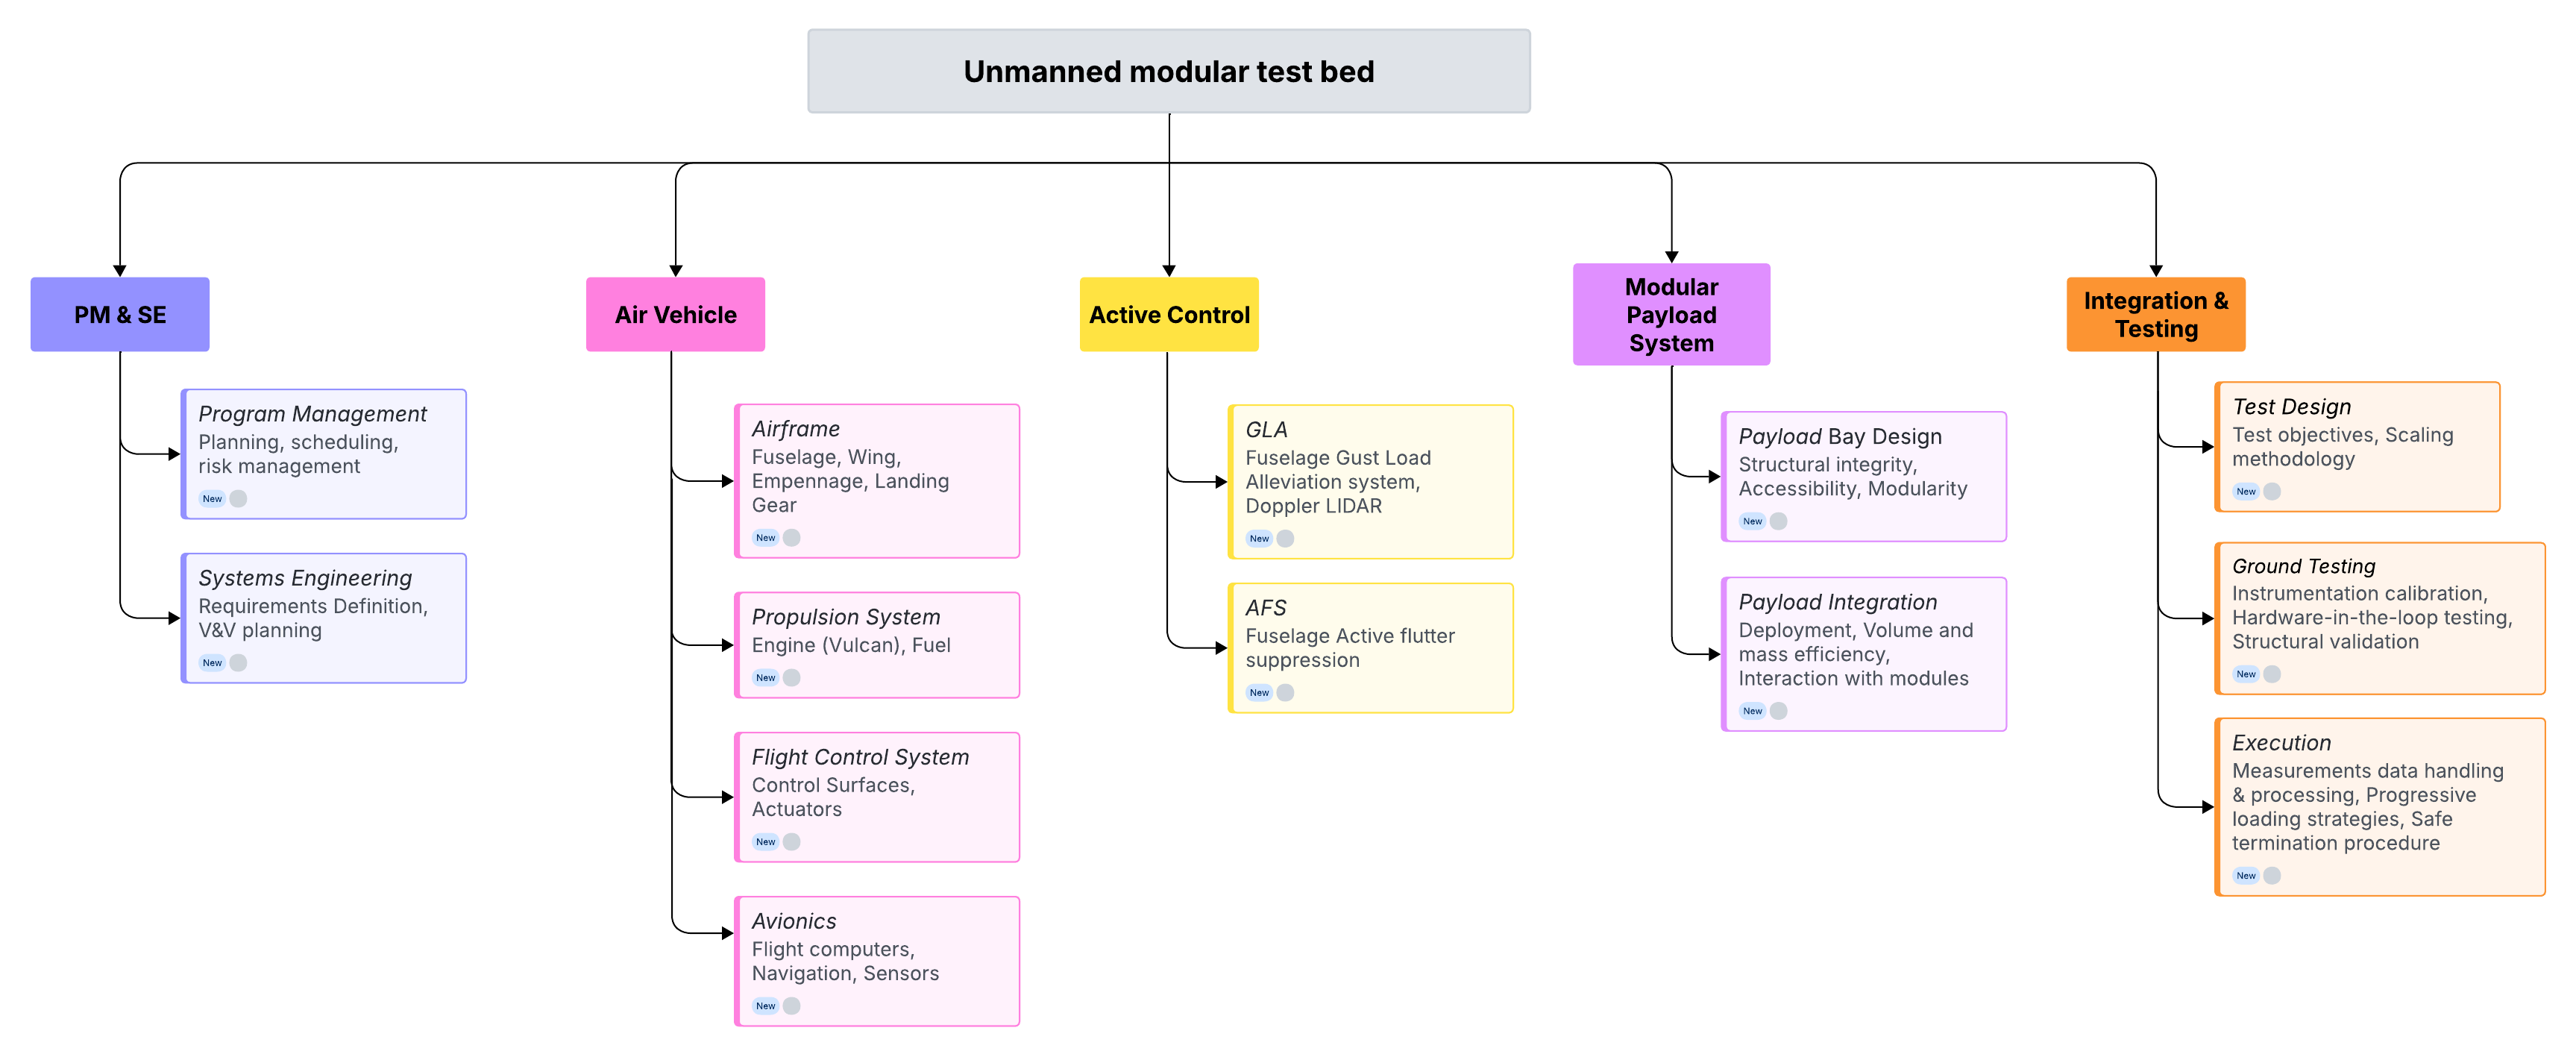
\includegraphics[width=1.1\linewidth]{figures/Work breakdown structure (WBS).png}
    \caption{Work Breakdown Structure of the Unmanned Flying Laboratory}
    \label{fig:placeholder}
\end{figure}



\section{Schedule (Gantt Chart)}
